\documentclass[xcolor=dvipsnames]{beamer}

\usepackage[utf8]{inputenc}
\usepackage[english]{babel}
\usepackage{url}
\usepackage{lmodern}
\usepackage{listings}
\usepackage{graphicx}
\usepackage{xcolor}
\usepackage{textcomp} 
\usepackage{hyperref}
\usepackage{subcaption}
\usepackage[T1]{fontenc}

\usepackage{color}
 
\definecolor{dkgreen}{rgb}{0,0.6,0}
\definecolor{gray}{rgb}{0.5,0.5,0.5}
\definecolor{mauve}{rgb}{0.58,0,0.82}
 
\lstset{
  language=c++,                % the language of the code
  basicstyle=\footnotesize,       % the size of the fonts that are used for the code
  numbers=left,                   % where to put the line-numbers
  numberstyle=\tiny\color{gray},  % the style that is used for the line-numbers
  stepnumber=1,                   % the step between two line-numbers. If it's 1, each line 
                                  % will be numbered
  numbersep=5pt,                  % how far the line-numbers are from the code
  backgroundcolor=\color{white},      % choose the background color. You must add \usepackage{color}
  showtabs=false,                 % show tabs within strings adding particular underscores
  frame=single,                   % adds a frame around the code
  rulecolor=\color{black},        % if not set, the frame-color may be changed on line-breaks within not-black text (e.g. comments (green here))
  tabsize=2,                      % sets default tabsize to 2 spaces
  captionpos=b,                   % sets the caption-position to bottom
  breaklines=true,                % sets automatic line breaking
  breakatwhitespace=false,        % sets if automatic breaks should only happen at whitespace
  title=\lstname,                   % show the filename of files included with \lstinputlisting;
                                  % also try caption instead of title
  keywordstyle=\color{blue},          % keyword style
  commentstyle=\color{dkgreen},       % comment style
  stringstyle=\color{mauve},         % string literal style
  morekeywords={initial\_state, final\_state, nextstate},
  extendedchars=true,
  literate={é}{{\'e}}1 {è}{{\`e}}1 {à}{{\`a}}1 {ç}{{\c{c}}}1 {œ}{{\oe}}1 {ù}{{\`u}}1
  {É}{{\'E}}1 {È}{{\`E}}1 {À}{{\`A}}1 {Ç}{{\c{C}}}1 {Œ}{{\OE}}1 {Ê}{{\^E}}1
  {ê}{{\^e}}1 {î}{{\^i}}1 {ô}{{\^o}}1 {û}{{\^u}}1
}


\setbeamertemplate{footline}{\hspace*{.5cm}\scriptsize{\insertauthor\hspace*{50pt} \hfill\insertframenumber\hspace*{.5cm}}}

\setbeamertemplate{section in toc}{%
\textcolor{MidnightBlue}{$\blacktriangleright$ \inserttocsection}
}

\usecolortheme{seahorse}
\usecolortheme{rose}
\useoutertheme{infolines}

\usecolortheme[named=SkyBlue]{structure}
\setbeamercolor{block title}{fg=MidnightBlue}

\AtBeginSection[]
{
  \begin{frame}<beamer>{Content}
    \tableofcontents[currentsection,hideothersubsections]
  \end{frame}
} 

\title{\textsc{neev}: Event-driven networking library}
\subtitle{FOSDEM 2014}
\author[Pierre \textsc{Talbot}]{Pierre \textsc{Talbot} \texttt{(ptalbot@hyc.io)}}
\institute[UMPC]{University of Pierre et Marie Curie}
\date[]{2014, February 1}

\begin{document}
\maketitle

\section{Introduction}

\subsection{Add-on server}
\begin{frame}
\frametitle{Add-on server}

\begin{figure}[p]
  \centering
  \begin{subfigure}[b]{0.3\textwidth}
    
\includegraphics[scale=0.3]{images/wesnoth-logo.png}
  \end{subfigure}
  \qquad \qquad \quad
  \begin{subfigure}[b]{0.3\textwidth}
    
\includegraphics[scale=0.1]{images/gsoc2013.jpg}
  \end{subfigure}
\end{figure}

\begin{enumerate}
\item Manage user-made contents (UMC).
\item Dependencies resolution.
\item Synchronization with translation.
\end{enumerate}

\begin{block}{}
I didn't even finish (1).
\end{block}
\end{frame}

\subsection{About me}
\begin{frame}
\frametitle{About me}

\begin{itemize}
\item Belgian (French side).
\item Still a student, at the University Pierre et Marie Curie in Paris.
\item Interest in software engineering, language design and concurrency.
\end{itemize}

\begin{block}{Open-source involvement}
\begin{itemize}
\item \textbf{Boost C++ library} Working on Boost.Check and Boost.Expected
\item \textbf{Wesnoth} The add-on server (UMCD).
\end{itemize}
\end{block}
\end{frame}

\subsection{About \textsc{neev}}

\begin{frame}
\frametitle{What is \textsc{neev}?}

\begin{itemize}
\item Generic code extracted from UMCD and packaged as a library.
\item Tons of changes since.
\item \textsc{neev} stands for "Network events".
\end{itemize}

\begin{block}{Details}
\begin{itemize}
\item Host on Github: \url{https://github.com/ptal/neev}
\item Licensed under the Boost software license.
\item Currently you need the latest Boost version (1.55) and C++11.
\end{itemize}
\end{block}
\end{frame}

\begin{frame}
\frametitle{Which games?}

\begin{itemize}
\item Best suited for turn-based games.
\item We might add support later for real-time games.
\end{itemize}

\begin{itemize}
\item Not limited to game application.
\end{itemize}

\end{frame}

\section{Neev library}

\subsection{Neev in a nutshell}
\begin{frame}
\frametitle{Neev in a nutshell}

\begin{block}{Traits}
\begin{itemize}
\item Event-driven
\item Asynchronous
\item Extensible
\end{itemize}
\end{block}

Before diving into \textsc{neev}, let's see how Boost.Asio works.
\end{frame}

\subsection{Boost.Asio}

\begin{frame}
\frametitle{Boost.Asio in a really thin nutshell}

\begin{block}{Example}
\begin{enumerate}
\item You initiate an asynchronous operation on a socket.
\item When it finishes, the result is put onto a completion queue.
\item And the proactor dispatches the result to the completion handler.
\end{enumerate}
\end{block}

It's easier to see Boost.Asio as a producer-consumer queue.
\end{frame}

\subsection{Task queue simulation}
\begin{frame}
\frametitle{Start with empty queue}
\begin{figure}[p]
  \centering
  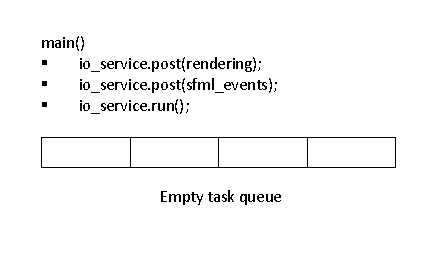
\includegraphics{images/queue-frame1.pdf}
\end{figure}
\end{frame}

\begin{frame}
\frametitle{Push onto the queue}
\begin{figure}[p]
  \centering
  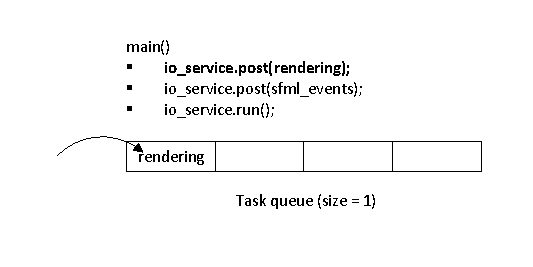
\includegraphics{images/queue-frame2.pdf}
\end{figure}
\end{frame}

\begin{frame}
\frametitle{Push onto the queue}
\begin{figure}[p]
  \centering
  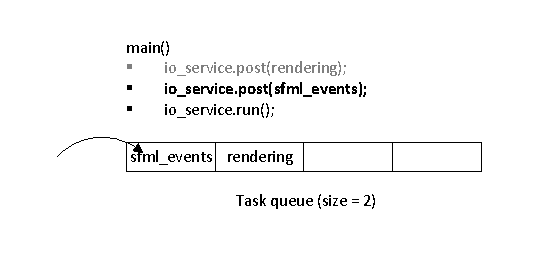
\includegraphics{images/queue-frame3.pdf}
\end{figure}
\end{frame}

\begin{frame}
\frametitle{Pop from the queue}
\begin{figure}[p]
  \centering
  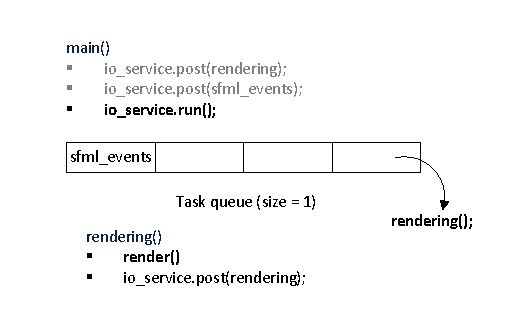
\includegraphics{images/queue-frame4.pdf}
\end{figure}
\end{frame}

\begin{frame}
\frametitle{Execute a task}
\begin{figure}[p]
  \centering
  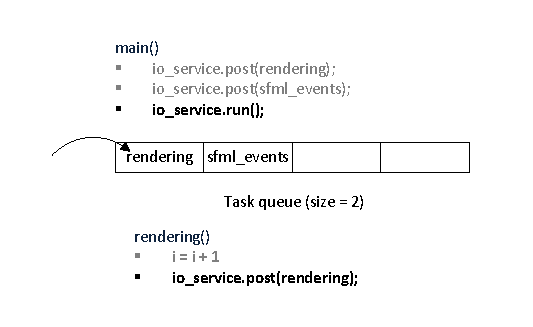
\includegraphics{images/queue-frame5.pdf}
\end{figure}
\end{frame}

\begin{frame}
\frametitle{Pop from the queue}
\begin{figure}[p]
  \centering
  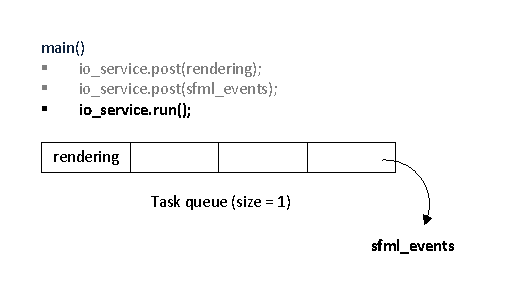
\includegraphics{images/queue-frame6.pdf}
\end{figure}
\end{frame}

\begin{frame}
\frametitle{Start two threads}
\begin{figure}[p]
  \centering
  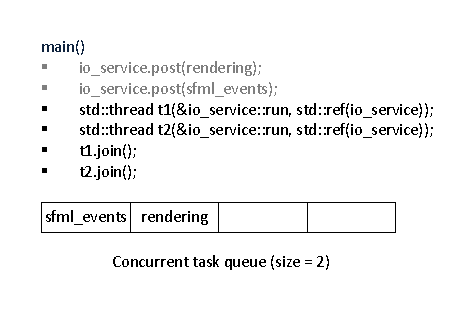
\includegraphics{images/queue-frame7.pdf}
\end{figure}
\end{frame}

\begin{frame}
\frametitle{Concurrently execute threads}
\begin{figure}[p]
  \centering
  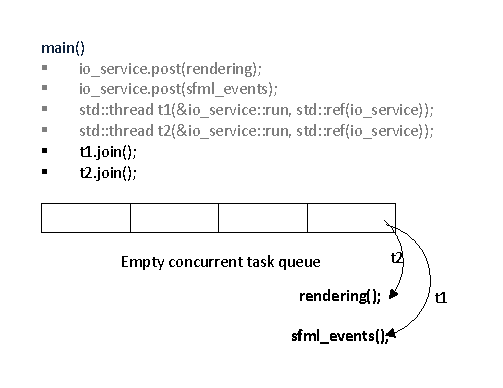
\includegraphics{images/queue-frame8.pdf}
\end{figure}
\end{frame}

\section{Example}
\subsection{Client}
\begin{frame}[fragile]
\frametitle{I'm the client, how do I connect?}
\begin{lstlisting}
void handler(const socket_ptr& socket);

int main()
{
  boost::asio::io_service io_service;
  neev::client client(io_service);
  client.on_event<neev::connection_success>(handler);
  client.async_connect("localhost", "12222");
  io_service.run();
  return 0;
}
\end{lstlisting}
\end{frame}

\begin{frame}
\frametitle{Client connection events}
\begin{itemize}
  \item \textbf{try\_connecting\_with\_ip}: \lstinline{void handler(const std::string&);}
  \item \textbf{connection\_success}: \lstinline{void handler(const socket_ptr&);}
  \item \textbf{connection\_failure}: \lstinline{void handler(const boost::system::error_code&);}
\end{itemize}
\end{frame}

\subsection{Server}
\begin{frame}[fragile]
\frametitle{How to launch the server?}
\begin{lstlisting}
void on_new_client(const socket_type& socket);

int main()
{
  basic_server server;
  server.on_event<new_client>(on_new_client);
  server.launch("12222");
  return 0;
}
\end{lstlisting}
\end{frame}

\begin{frame}
\frametitle{Server connection events}
\begin{itemize}
  \item \textbf{start\_success}: \lstinline{void handler(const endpoint_type&);}
  \item \textbf{new\_client}: \lstinline{void handler(const socket_ptr&);}
  \item \textbf{run\_exception}: \lstinline{void handler(const std::exception&);}
  \item \textbf{run\_unknown\_exception}: \lstinline{void handler();}
  \item \textbf{start\_failure}: \lstinline{void handler();}
  \item \textbf{endpoint\_failure}: \lstinline{void handler(const std::string&);}
\end{itemize}
\end{frame}

\subsection{Transfer}

\begin{frame}[fragile]
\frametitle{Simple position structure}
\begin{lstlisting}
struct Position
{
  std::int32_t x, y, z;

  template <class Archive>
  void serialize(Archive& ar, const unsigned int)
  {
    ar & x & y & z;
  }
};
\end{lstlisting}
\end{frame}

\begin{frame}[fragile]
\frametitle{Sending}
\begin{lstlisting}
void send_random_pos(const socket_type& socket)
{
  auto sender = neev::make_archive16_sender<no_timer>(
    socket, 
    make_random_position());

  sender->on_event<neev::transfer_complete>(handler);

  sender->async_transfer();
}
\end{lstlisting}
\end{frame}

\begin{frame}[fragile]
\frametitle{Receiving}
\begin{lstlisting}
void receive_random_pos(const socket_type& socket)
{
  auto receiver = make_archive16_receiver<Position,no_timer>(socket);
  
  receiver->on_event<transfer_complete>([=](){
    std::cout << receiver->data() << std::endl;});

  receiver->async_transfer();
}
\end{lstlisting}
\end{frame}

\begin{frame}
\frametitle{Transfer events}
\begin{itemize}
  \item \textbf{transfer\_complete}: \lstinline{void handler();}
  \item \textbf{transfer\_error}: \lstinline{void handler(const boost::system::error_code&);}
  \item \textbf{transfer\_on\_going}: \lstinline{void handler(std::size_t, std::size_t);}
  \item \textbf{chunk\_complete}: \lstinline{void handler(events_subscriber_view<transfer_events>);}
\end{itemize}
\end{frame}

\subsection{Buffers}

\begin{frame}
\frametitle{Buffers}

\begin{block}{Different kinds}
\begin{itemize}
  \item Fixed-size buffers (e.g. text data, files, ...).
  \item Non-delimited buffers (e.g. JSON, XML, binary data).
\end{itemize}
\end{block}

\begin{figure}[p]
  \centering
  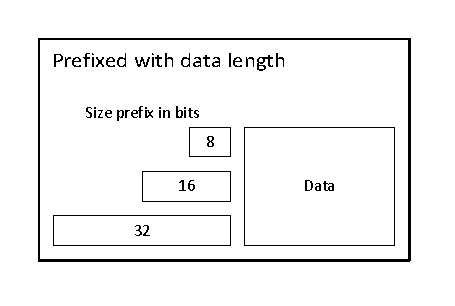
\includegraphics{images/fixed-buffer.pdf}
\end{figure}

\end{frame}

\begin{frame}
\frametitle{Non-delimited buffers}

\begin{figure}[p]
  \centering
  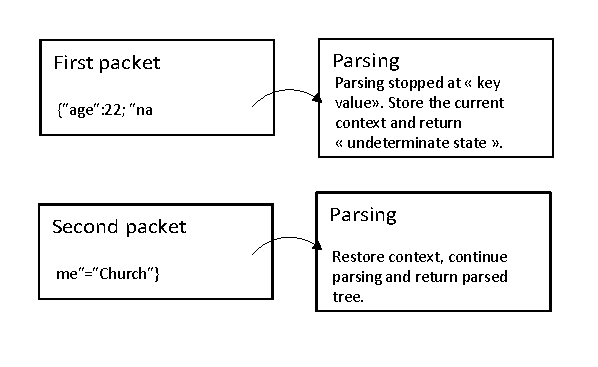
\includegraphics{images/parsing-buffer.pdf}
\end{figure}

\end{frame}

\subsection{Events}

\begin{frame}
\frametitle{Why event-driven?}

\begin{itemize}
  \item Clean design.
  \item Less code and better factorization.
  \item Compositionality.
\end{itemize}

\begin{block}{Spaghetti code?}
\begin{itemize}
  \item It might be if we relaunched events inside event-handlers.
  \item Nothing in the current design indicates that you should do that.
\end{itemize}
\end{block}
\end{frame}

\begin{frame}
\frametitle{Why asynchronous?}

\begin{itemize}
\item Inherits the pros and cons of Boost.Asio
\end{itemize}

\begin{exampleblock}{Advantages}
\begin{itemize}
  \item Portability and efficiency (use native asynchronous I/O API if available).
  \item Decoupling threads from concurrency.
  \item Scalability.
\end{itemize}
\end{exampleblock}

\begin{alertblock}{Disadvantages}
\begin{itemize}
  \item Program complexity (separation in time and space between operation initiation and completion).
  \item Nearly everything allocated on the heap.
\end{itemize}
\end{alertblock}

\end{frame}


\section{And next?}

\begin{frame}
\frametitle{More buffer}

\begin{block}{Plenty of work}
\begin{itemize}
\item XML;
\item JSON;
\item WML;
\item True binary data.
\end{itemize}
\end{block}

\begin{itemize}
\item Support for existing XML/JSON libraries.
\end{itemize}
\end{frame}

\begin{frame}
\frametitle{More low-level protocols support}

\begin{itemize}
  \item UDP support
  \item SSL transmission
  \item Simple heartbeat protocol
\end{itemize}
\end{frame}

\begin{frame}
\frametitle{And finally...}

\begin{itemize}
  \item Allocator support.
  \item More documentation, examples and tests.
  \item Concurrent development with the Wesnoth add-on server.
\end{itemize}

\begin{exampleblock}{Contributors}
Do not hesitate to contribute ;-)
\end{exampleblock}
\end{frame}

\begin{frame}
\frametitle{Questions}
\begin{center}
\Large{Feel free to ask any questions.}
\end{center}
\begin{figure}[p]
  \centering
  \includegraphics[scale=0.6]{images/question.jpeg}
\end{figure}
\end{frame}

\begin{frame}
\begin{center}
\Large{Thanks for your attention!}
\end{center}
\end{frame}


\end{document}
